%!TEX root = ../dissertation.tex
\chapter{Some extra stuff}
\label{AppendixA}


\section{Molding equipments}

\paragraph{Female mold:}
It consists of a cylinder of radius $R_{cylinder}=30$ mm  hollowed out to produce a half a sphere imprint of radius $R_{out}=25$ mm and a height of $h = 30$ mm (see fig.\ref{fig:female_mold}). The concavity is where the casting material is poured.
A groove was added to store any potential material surplus. Two female molds are necessary for the casting operation.
\begin{figure}[H] %
	\centering%
		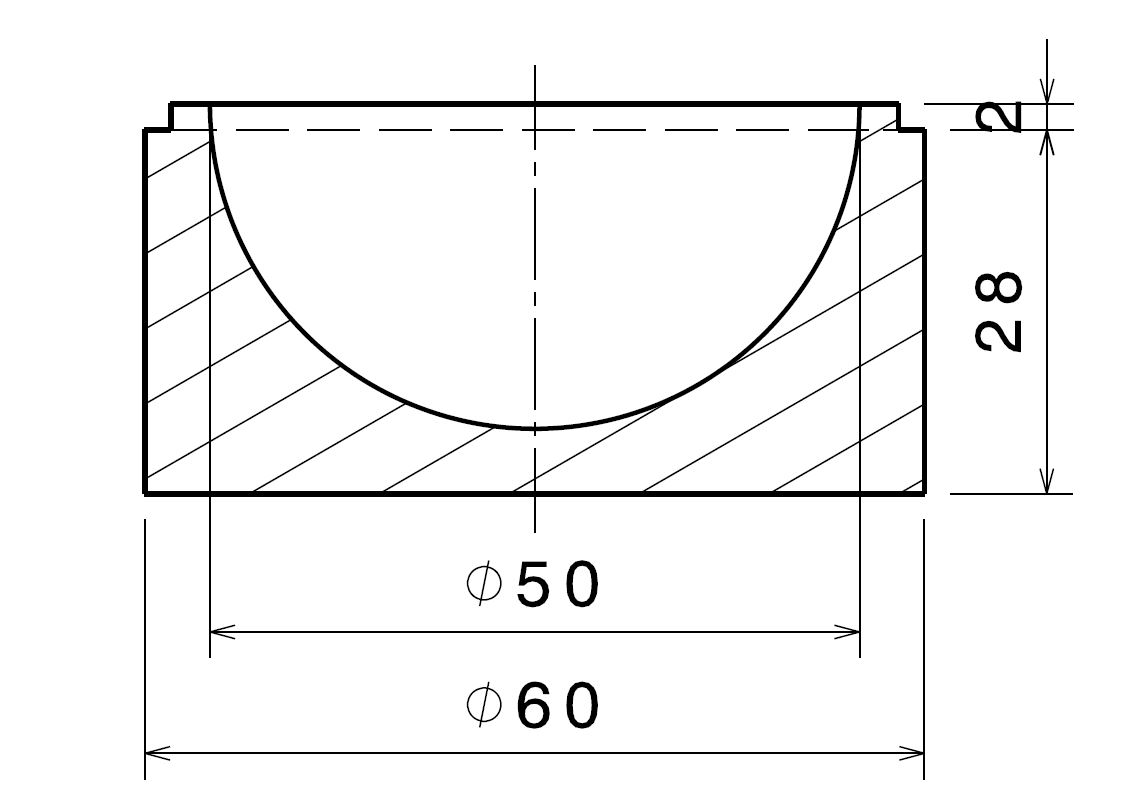
\includegraphics[width=0.48\textwidth]{figures/Chapter_1/female_mold.jpg}%
		\caption{Longitudinal section of the female mold}%
		\label{fig:female_mold}%
\end{figure}


\paragraph{Translation guide sleeve:}
It is a hollow cylinder with an inner radius $R_{in} = R_{cylinder} = 30$ mm, and a thickness of $5$ mm. where the female mold is slid in. It is slightly higher than the female mold by $5$ mm. One extremity is provided with an inner chamfer of 5\textdegree which ensures the concentricity between the female mold and the male mold.
\begin{figure}[H] %
	\centering%
  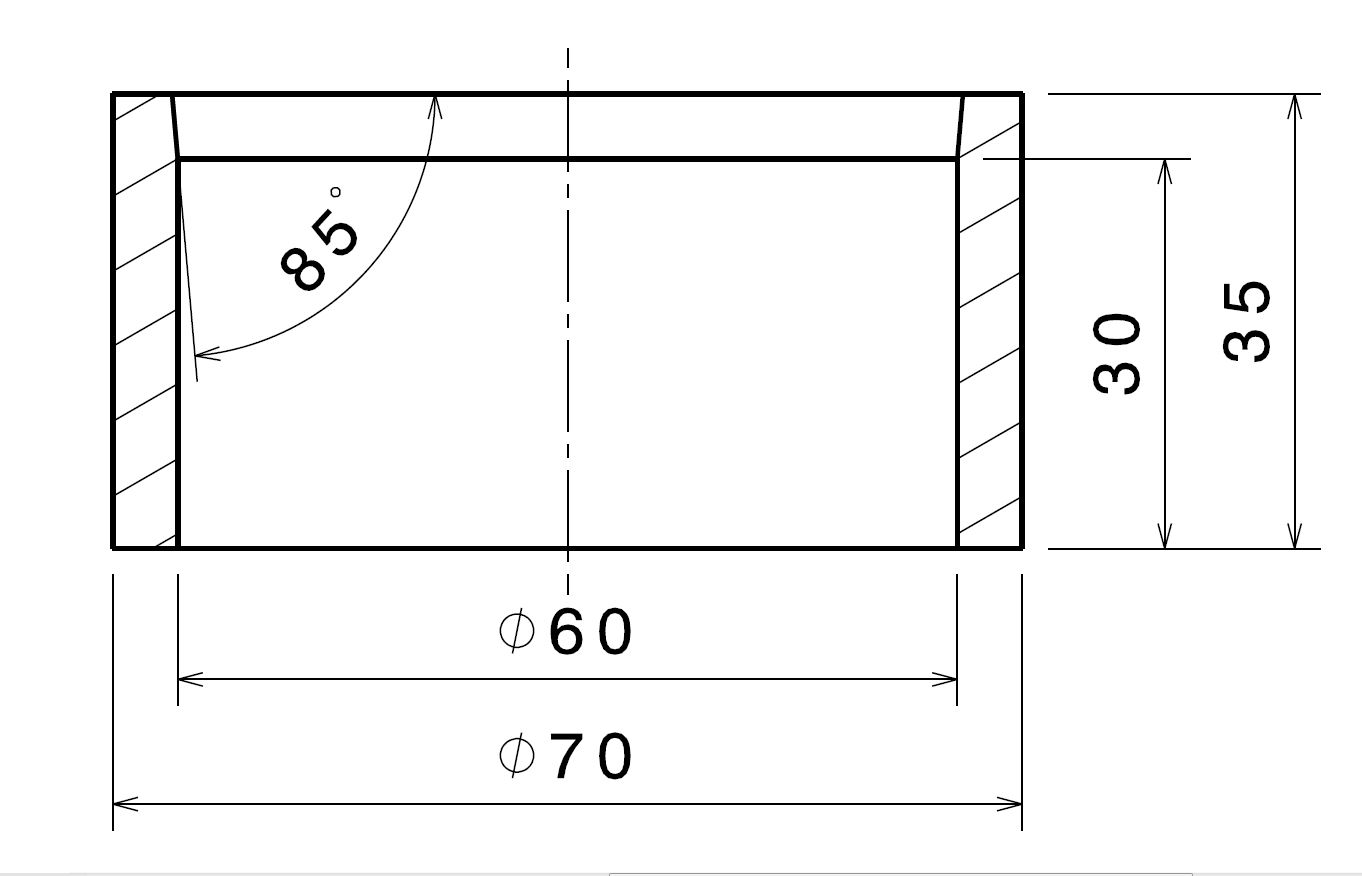
\includegraphics[width=0.48\textwidth]{figures/Chapter_1/sleeve_translation.jpg}
  \caption{longitudinal section of the sleeve}%
	\label{fig:sleeve_1}%
\end{figure}

\paragraph{Male mold:}
Figure \ref{fig:male_mold} shows the design of the male mold which consists of half a sphere of radius $R_{int}<R_{out}$, which is changed to cast different thicknesses. It is supplied with a shouldering which acts as a travel stop, its flanks have a slight angle of 5 providing a translation guide and preventing an over-center locking in combination with the guiding sleeve previously presented. The cylindrical part over the shouldering helps manipulating the mold during the casting process. Three radii have been used: $R_{int} = 18.5 mm, 20 mm, 23 mm$. 
\footnote{All the molding parts presented are made of Aluminum "`Fortal"'. The female and male molds were machined using a CNC (computerized numerical control)  machine and with a precision of $tol =\pm 0.01$ mm. The surface roughness obtained was of $R_a = 0.04$ which indicates a very good finishing.
This choice of manufacturing was unavoidable since no other alternative could produce spherical shapes with such a precision.}
\begin{figure}[H] %
	\centering%
  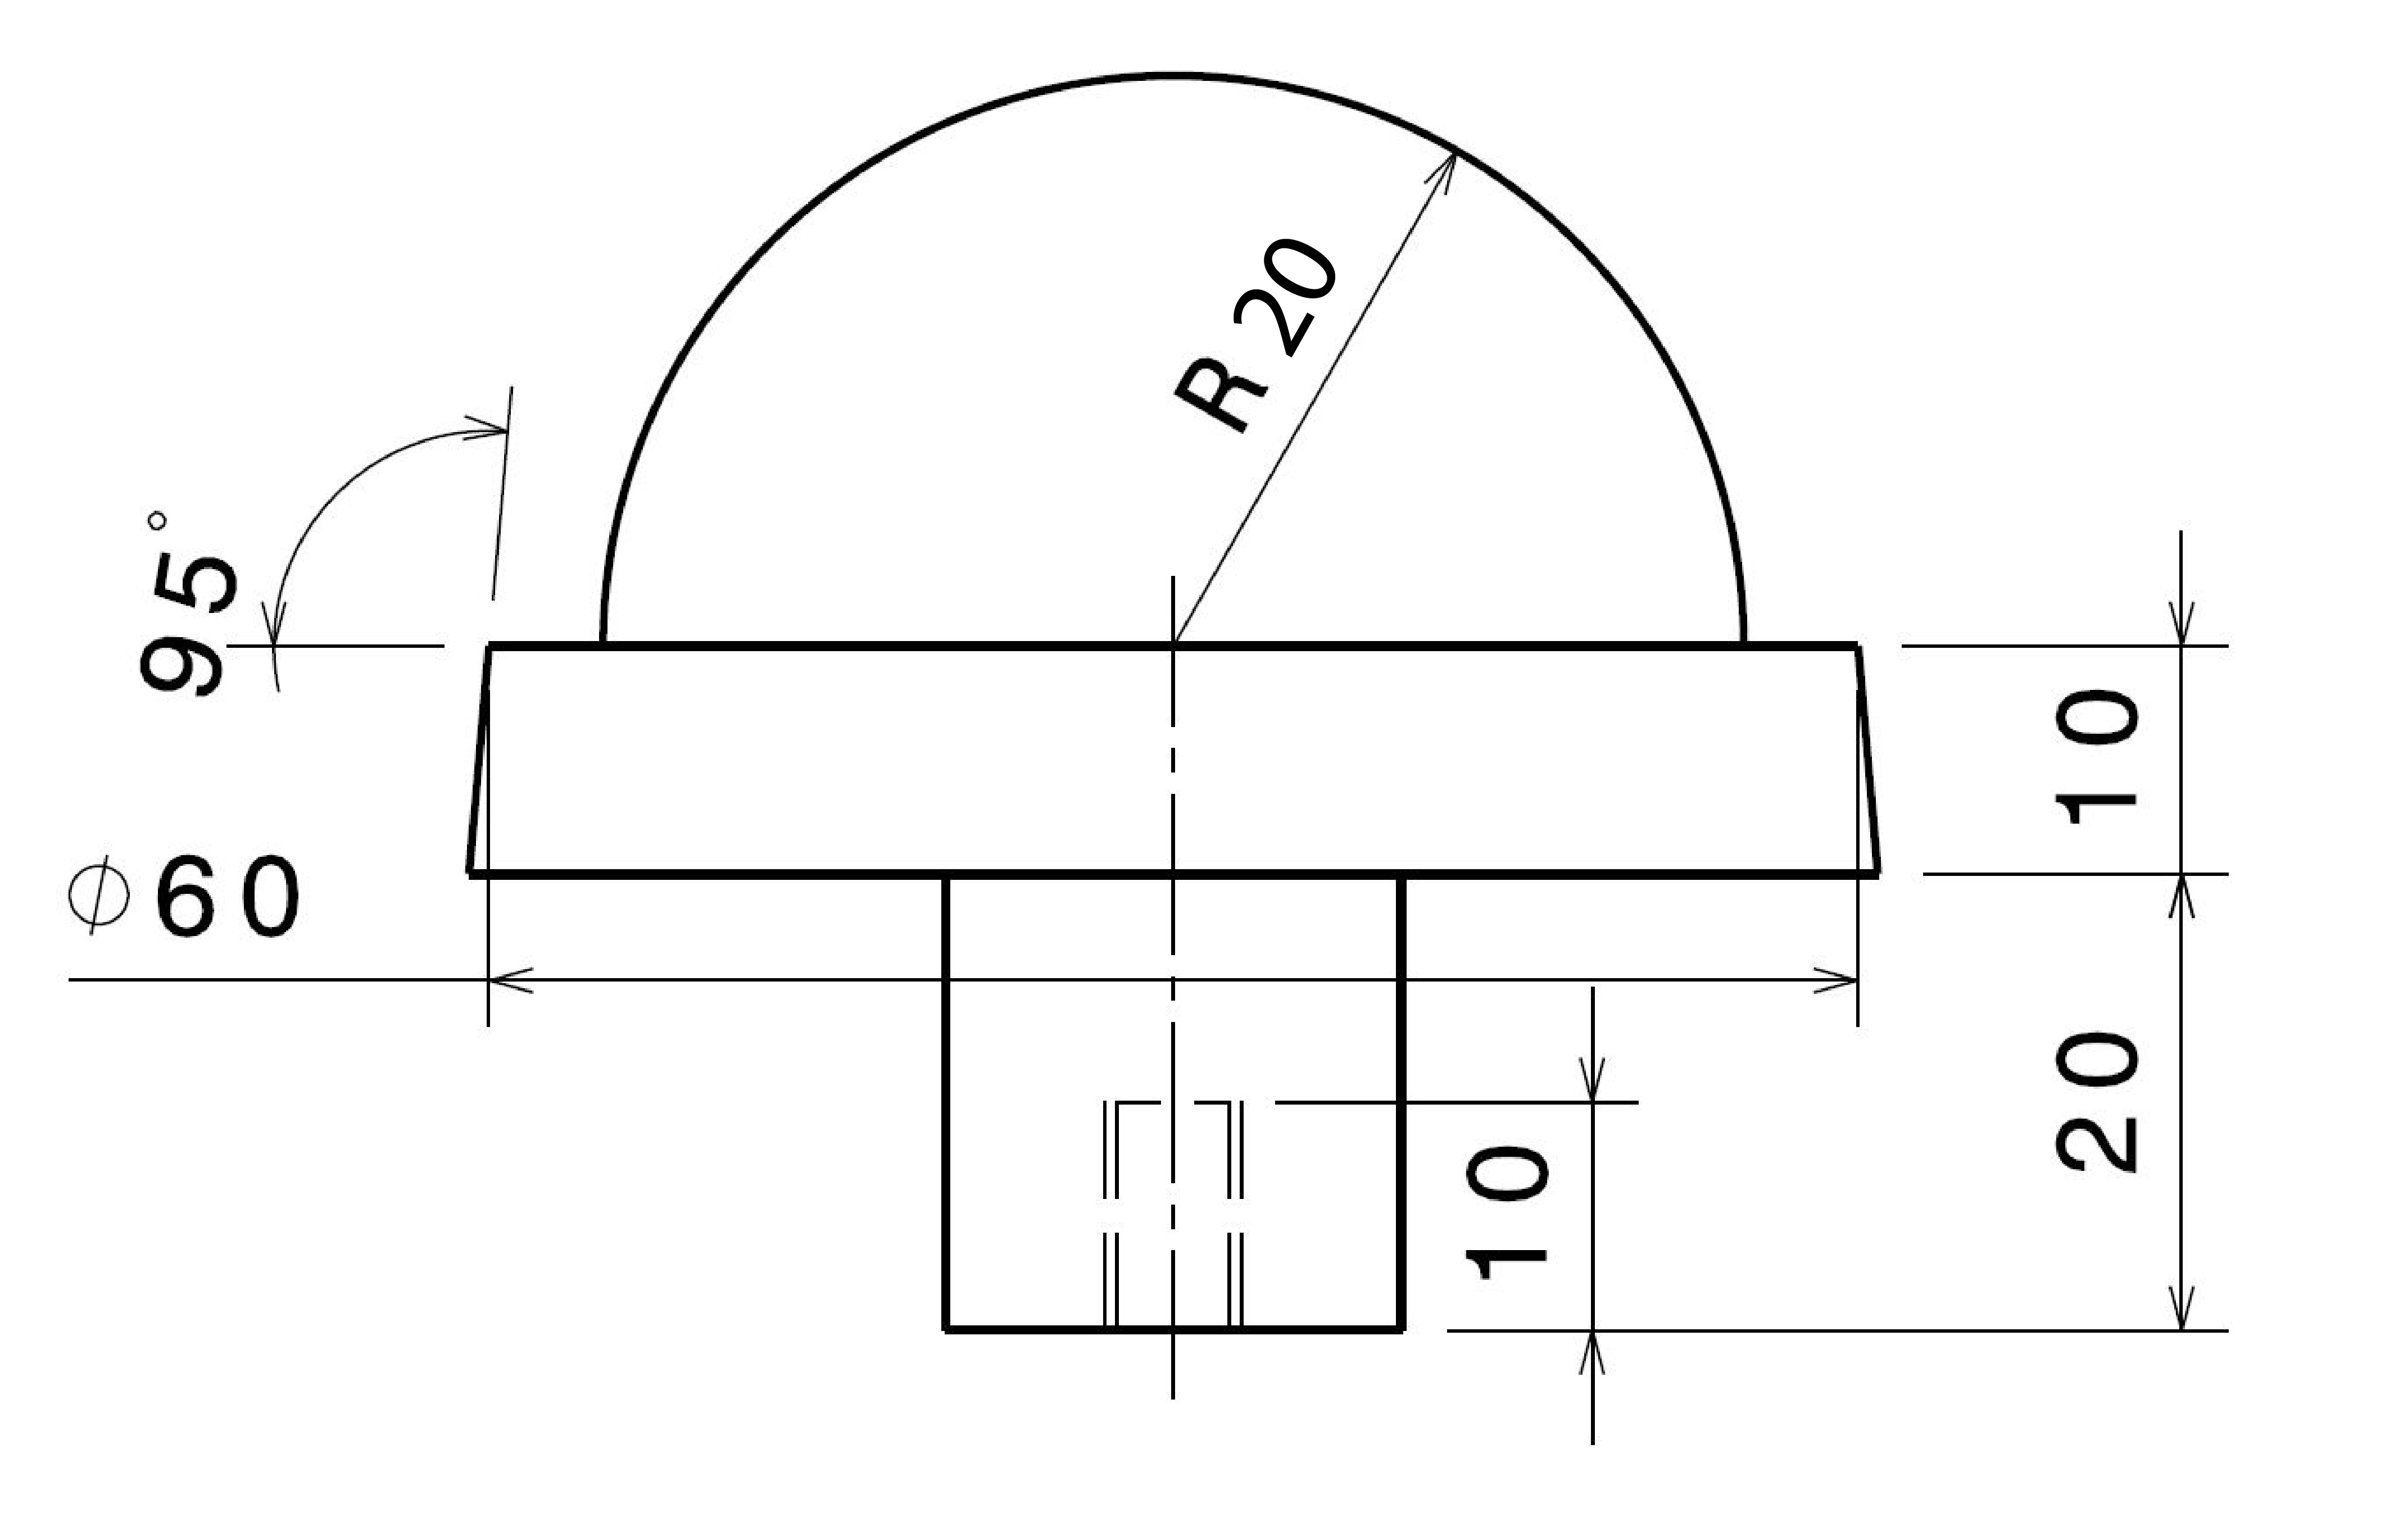
\includegraphics[width=0.48\textwidth]{figures/Chapter_1/male_mold.jpg}
	\caption{Front view of an example of the male molds used}
	\label{fig:male_mold}
\end{figure}

\paragraph{Gluing sleeve:}
It is a hollow cylinder with an inner radius $R_{in} = R_{cylinder} = 30$ mm, a thickness of $5$ mm and a height of $50$ mm. It is used during the gluing process where the female molds containing the two halves of the sphere, are faced to each other and slid inside the gluing sleeve, to ensure the concentricity.

\paragraph{Mechanical press:}
It's a simple press consisting of two metallic plates supplied with a set of threaded rods and hexagonal nuts used to apply pressure over female/male molds during the casting step, preventing air bubbles from getting trapped, during the casting step. It is also used during the gluing step on the female/female molds, to ensure the contact between the two half spheres to be glued together.

\paragraph{Pasta machine:}
This machine (fig\ref{fig:pasta_maker}) consists in two rotating cylinders, with an adjustable inter-space. It was used to produce thin layers of a polymeric material.
\begin{figure}[H] %
	\centering%
  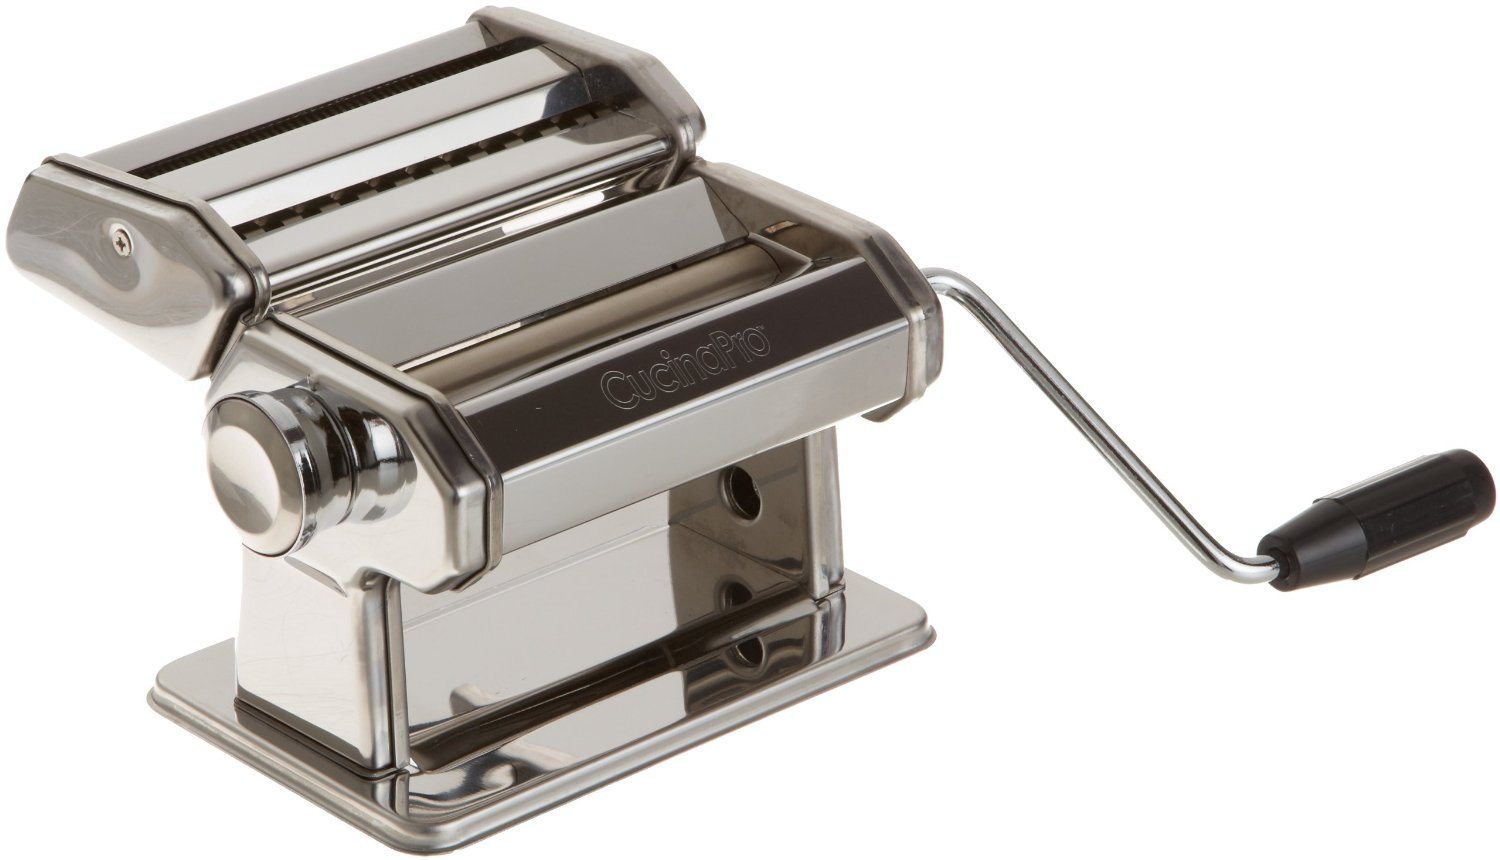
\includegraphics[width=0.48\textwidth]{figures/Chapter_1/rolling_machine.png}
	\caption{Pasta maker}
	\label{fig:pasta_maker}
\end{figure}





\section{Dragon skin\textregistered 30 molding protocol}
\paragraph{Half shell casting}
To produce a shell with a certain thickness $d$, made of Dragon skin\textregistered 30 material, these are the steps we followed: 
\begin{enumerate}
	\item Begin by determining the mass of a shell with a outer radius of $R_{out}= 25 mm$ and a thickness $d$ which gives an internal radius $R_{int} = R_{out}-d$

	\item In a beaker, weigh 50\% of the shell mass of component A which is the silicon polymer chain. We stir thoroughly and add 50\% of the shell mass of component B, which constitutes the cross-linking agent, we stir thoroughly.
	\item The mixture is then degassed using a vacuum pump.
	\item The female and male are cleaned using acetone and 50\% of the degassed mixture is poured in each one of the two female molds.
	\item We degas again to make sure no air was entrapped during the previous step.
	\item Each female mold is slid in the translation guide sleeve and the male mold with an internal radius $ R_{int}$ which corresponds to the desired thickness $d$ defined as $d = R_{out}-R_{int}$, is gently slid inside the female mold to prevent air from getting trapped.
	\item The female-male molds assembly is then pressed and locked using the press.\footnote{This step is necessary to ensure that no bubbles get trapped during the assembly.}
	\item The press is then put into an oven at 65°C to speed up the cross-linking process reducing it from 16 hours to only 20 minutes.
	
\end{enumerate}

\paragraph{Half spheres gluing:}
Once the two halves of a hollow sphere of the desired thickness $d$, are cast. Next step is to glue the two halves together to obtain a complete hollow sphere.
This part is critical: if the sewing is weak, it will tear apart during the buckling phase. if the sewing is thick, it means that the shape is no longer spherical. If the gluing material is not the same, we lose the homogeneity of the material and potentially create a weak zone at the sewing.
\paragraph{} 
To efficiently glue the two halves and avoid the problems stated previously, we used the same material to perform the gluing, but for that it was necessary to decrease the viscosity of the mixture and enhance its wetting properties. For this purpose, we mixed Pentane which is an organic solvent \cite{NgLee2003} with the highest solubility parameter for PDMS, assuming it would also work well for the Dragon skin\textregistered 30 material .
The following describes the protocol of gluing:
\begin{enumerate}
	\item Prepare 10g of a mixture A+B of the Dragon skin\textregistered 30 and degas it.
	\item Add 5 ml of "`Pentane"' to the mixture and stir to obtain a diluted mixture that is neither too liquid nor too viscous and pump the resulting liquid inside a syringe.
	\item Use an abrasive such as sandpaper over the gluing area of the two casts, to make the surface rougher.
	\item Put back each cast in the female mold and align it correctly so that the gluing area is horizontal.
	\item Pour uniformly a layer of the diluted mixture using the syringe needle on the gluing area of both casts.
	\item Put one female mold inside the gluing sleeve, facing upward then slide the second one facing downward until the two gluing areas are in contact.
	\item Ensure the contact by using the mechanical press and let the cross-linking happen at room temperature for 16 hours.\footnote{This time we don't use the oven to ensure that the pressure inside the spherical hollow shell is the atmospheric pressure.}
	\item After the curing time, the shell is produced and the last step is remove the residual thin skin circling around the sewing area.
\end{enumerate}



\section{AJO 121/122 molding protocol}
\paragraph{Half shell casting:}
To produce a shell with a certain thickness $d$, made of \emph{AJO 121} and \emph{AJO 122}, these are the steps we followed: 
\begin{enumerate}
	\item We begin by determining the mass of a shell with a outer radius of $R_{out}= 50 mm$ and a thickness $th$ which gives an internal radius $R_{int} = R_{out}-th$, The mass of a hollow sphere is given by the following formula:
		\[Mass_{shell} = \frac{4\pi}{3}\rho_{material} (R_{out}^3-R_{int}^3) \]

	\item We weigh the calculated mass from the paste-like material and divide it in two equal parts.
	\item Press each part at the center of the female mold.
	\item Each female mold is slid in the translation guide sleeve and the male mold corresponding to the desired $R_{int}$ is slid inside the female mold.
	\item The female-male molds assembly is then pressed and locked using the press.
	\item The press is then put into an oven at 115°C to trigger the vulcanization process, during 10 minutes.
	\item A post-curing at 200°C is needed to optimize the mechanical properties of the material, to evaporate remaining volatile substances (sub-products linked to the peroxide) and allow the sublimation of the 2,4 Dichlorobenzoic acid which manifests as a white powder at the surface of the material, at the end of the previous step.
\end{enumerate}

\paragraph{Half spheres gluing:}
After casting the two halves of the spherical capsule, the next step is to glue them together, but the gluing using the AJO materials was very challenging for different reasons. First, the paste-like nature of the material which was not soluble in any organic solvent without compromising the vulcanization agent already mixed with the raw polymer. It also made manipulating it harder, contrary to the liquid nature of the "`Dragon Skin\textregistered 30"'. Second, we were not able to glue together two flat surfaces, due to the fact that the cross-linking process reached a maximum with the prescribed time and temperature and leaving no room for an additional cross-linking.
After several trials, we came up with a protocol which allows to glue the two half spheres, following these steps:

\begin{enumerate}
	\item Two thin layers (0.1 mm) are prepared using the "`pasta maker"' machine (fig.\ref{fig:pasta_maker}). Their width is set to 10 mm and the length to $2\pi R_{out} \approx 157 mm$.
	\item Sandpaper is used over the gluing area of the two casts to make the surface rougher.
	\item Put back one cast in the female mold and align it correctly so that the gluing area is horizontal.
	\item Put uniformly a first layer on the gluing area of one cast and make sure it adhered to the surface, cut the residual width using a scalpel.
	\item Connect the remaining half (without the female mold) with the first and press to get and adhesion.
	\item Remove the female mold gently and roll the second layer around the sewing perimeter, taking care not to disconnect the two halves while doing so.
	\item Encapsulate the shell inside the two female molds and exert pressure using the mechanical press.
	\item Put the press inside the oven at 115°C for 10 minutes. Remove it and let it cool at room temperature.\footnote{The capsules produced using this protocol have an internal pressure close to $75\%$ of the atmospheric pressure.}
	\item The process ends by extracting the shell out of the female molds.
\end{enumerate}
\subsection{Material documentation}
\subsubsection{Dragon skin 30}
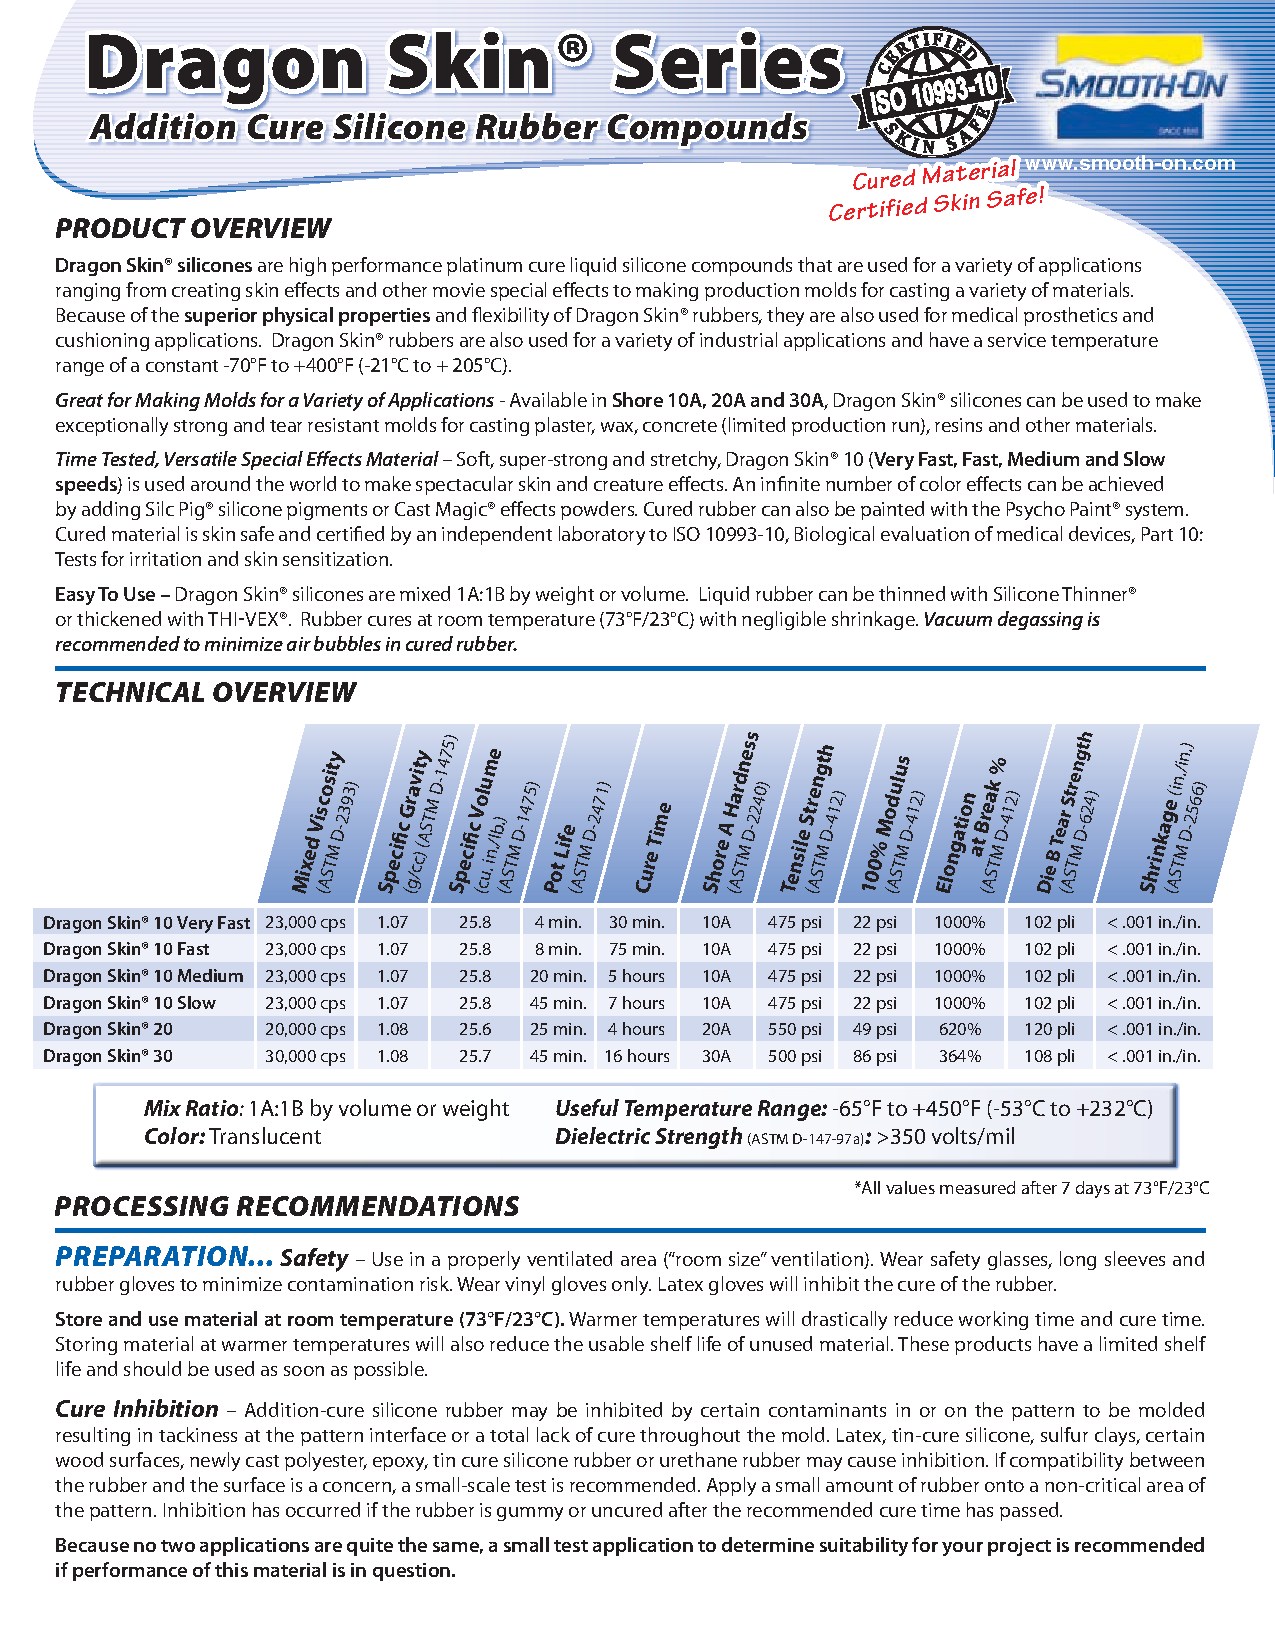
\includepdf[pages={1}]{Appendix/DRAGON_SKIN_SERIES_TB.pdf}
\subsubsection{AJO 121}
\paragraph{}
The commercial name is "`Bluesil MF 360"'.
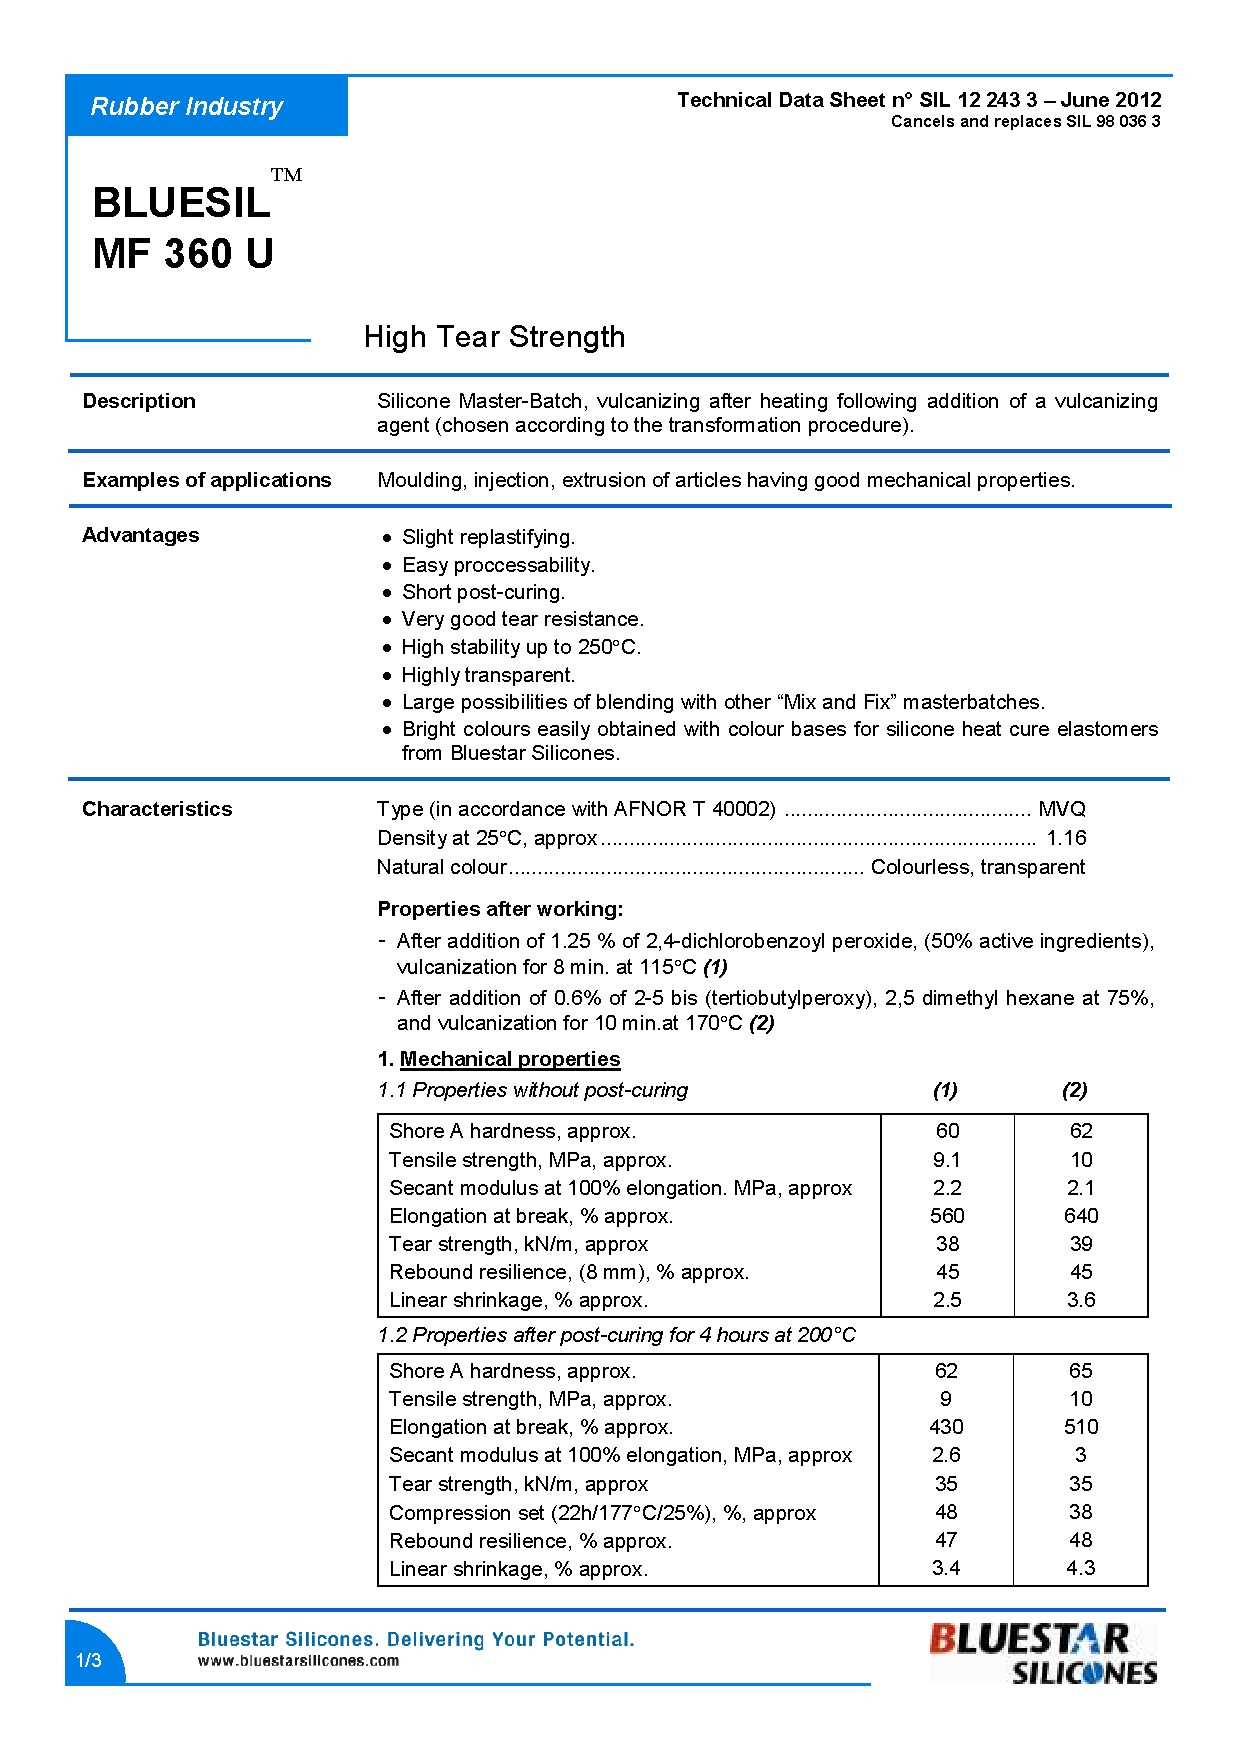
\includepdf[pages={1-2}]{Appendix/185100.pdf}
\subsubsection{AJO 122}
\paragraph{}
The commercial name is "`Bluesil MF 760"'.
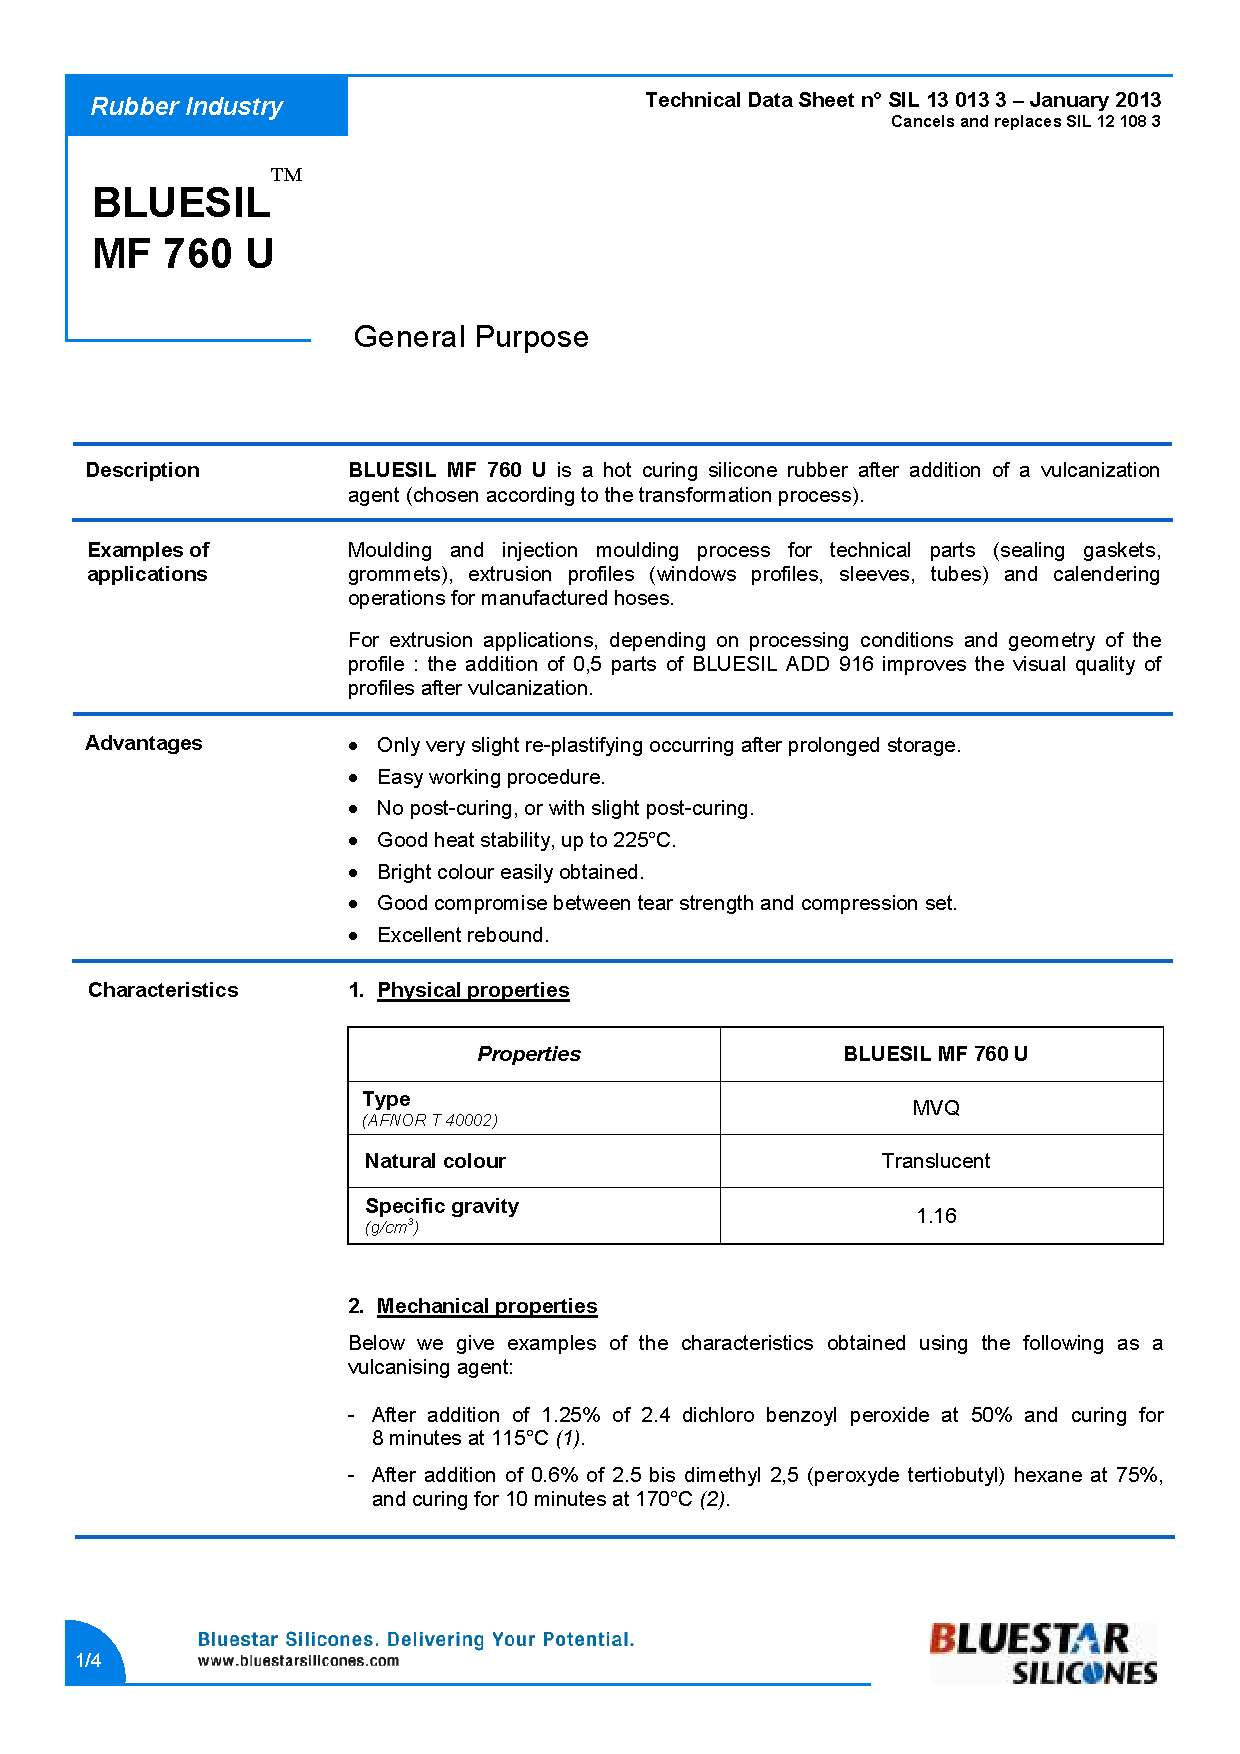
\includepdf[pages={1-3}]{Appendix/219488.pdf}

\section{Algorithm for fitting the external shape of the shell}
\paragraph{}
To fit the outer contour of the shell with a parametric curve, defined in the polar coordinates system, these operations were followed:
\begin{enumerate}
	\item Define an initial center 	$M_{c0} (x_{c0},y_{c0})$	to the polar coordinate system, as being the mean value of the experimental points constituting the ball shape.
	\begin{align*}
			x_{c0} &= \frac{\sum\limits_{i=1}^N x_i}{N} \\
			y_{c0} &= \frac{\sum\limits_{i=1}^N y_i}{N} \\
	\end{align*}
	Where $x_i$ and $y_i$	are the coordinates of the experimental points, and	$N$	being the number of points.
	\item Define an iterative process which minimizes the difference between a fitting parametric curve and the experimental points, where at each iteration, the 		following operations are performed: 
	
		\begin{enumerate}[label=\alph*)]
			\item Transform every experimental point from the Cartesian coordinates system  $M(x,y)$ to the polar coordinates system $M'(R,\theta)$  as follow:
				\begin{align*}
				R_{exp}(\theta)_i &=\sqrt{(x_i- x_c)^2+(y_i-y_c)^2}  \\
				\theta_{exp_i} &= \arctan(\frac{y_i-y_c}{x_i- x_c}) \\
				\end{align*}
				Where $x_c$ and $y_c$ are fitting parameters corresponding to the center of the polar coordinates, initialized by $M_{c0} (x_{c0},y_{c0})$.
			\item Evaluate the fitting parametric curve:
				\begin{align*}
					\tilde{R}(\theta)_i &=\sum\limits_{k=0}^M a_k \sin(\theta_{exp_i}-\theta_0)^k  \\
				\end{align*}
				for the fitting parameters $\theta_0$\footnote{$\theta_0$ represents the angle formed bet ween the symmetry axis of the experimental points and the y-axis.} 			 and $a_k$ coefficients, with $k={0,...,M}$, $M$ being the degree of the polynomial.
			\item Measure the distance $R_{exp}(\theta)_i-\tilde{R}_(\theta)_i$ and iterate.
		\end{enumerate}
	The minimization is done using $"`Levenberg-Marquardt"'$ method, commonly known as $"`least-squares"'$ minimization method.
	\item The iterative process stops when reaching a residual smaller than a given threshold.	
\end{enumerate}
\section{Frictionless rail}
\subsection{Technical details}
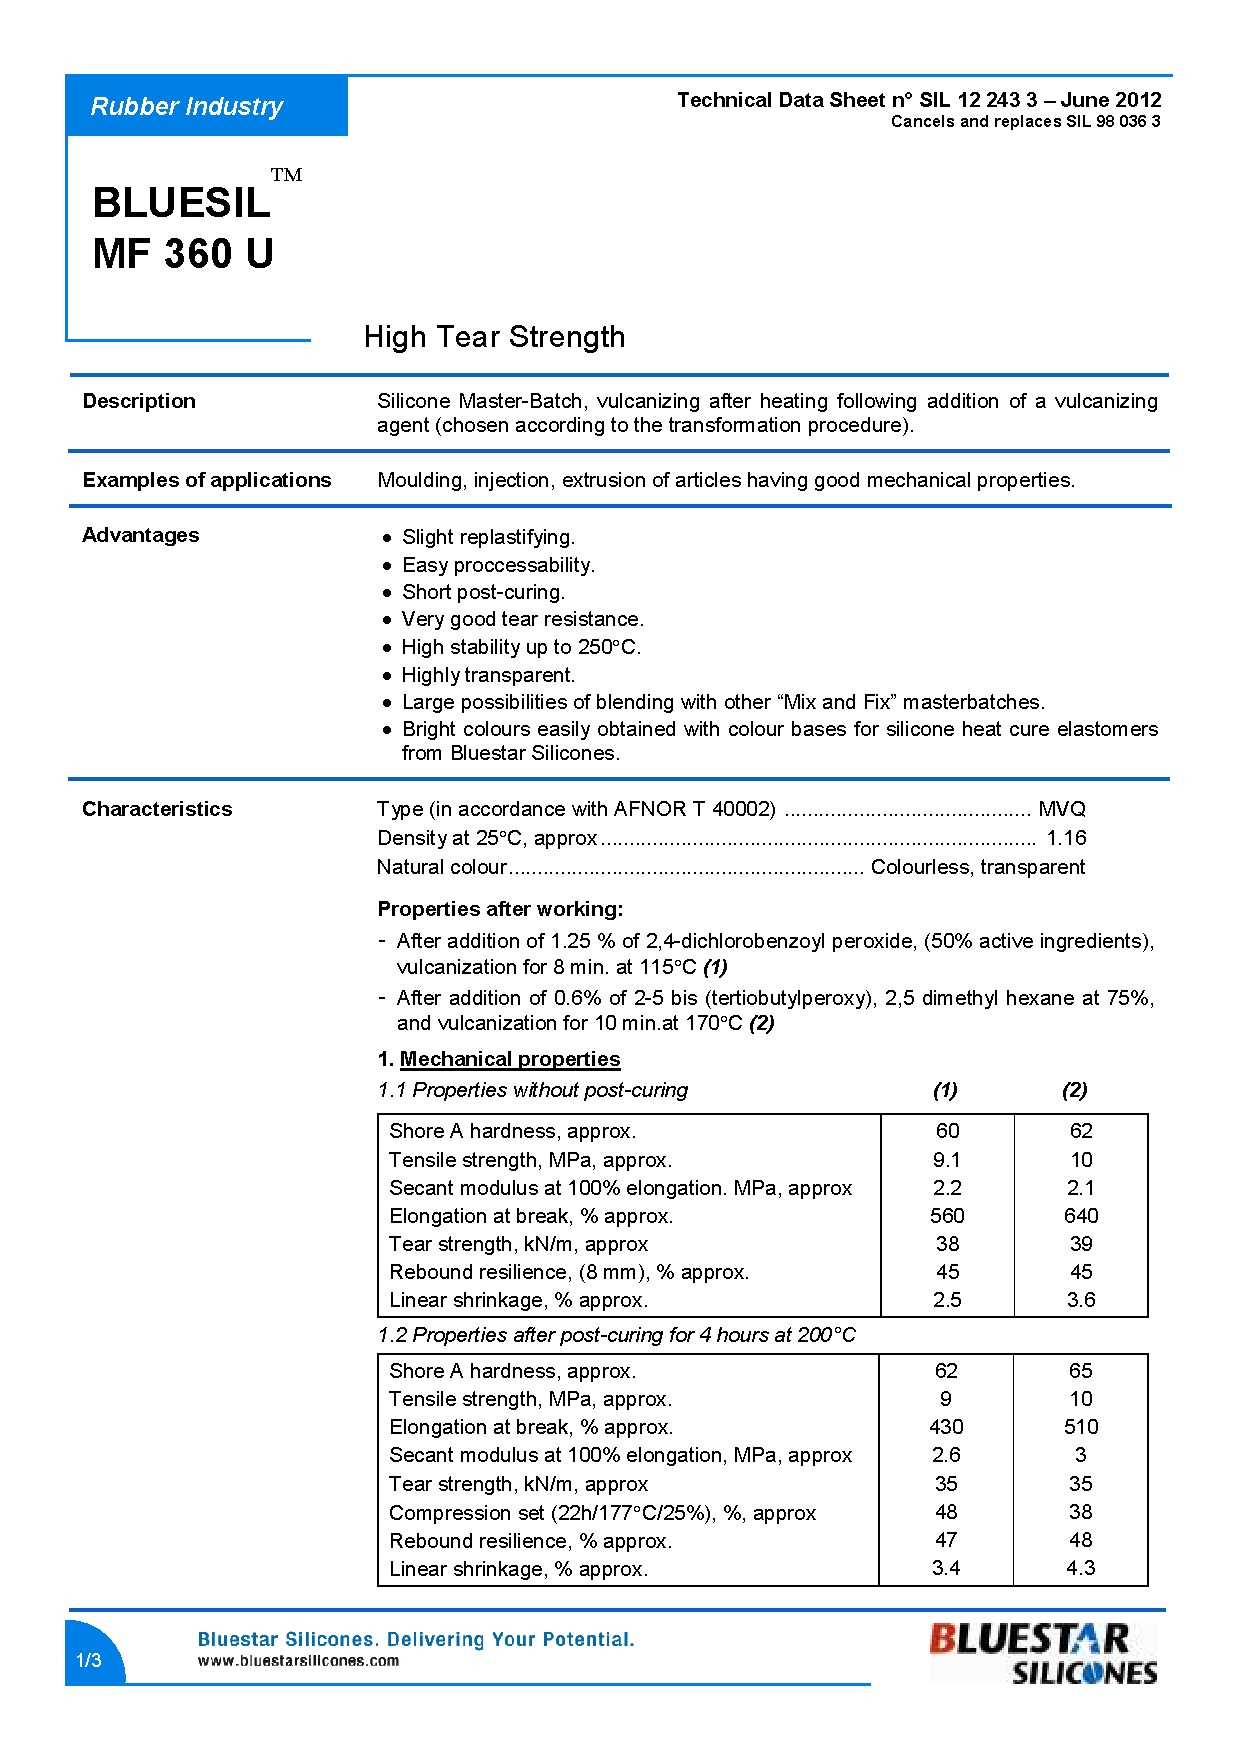
\includepdf[pages={1-2}]{Appendix/185100.pdf}
\section{PIV measurements}
\subsection{Davis image analysis parameters}

\begin{figure}[H] %
	\centering%
  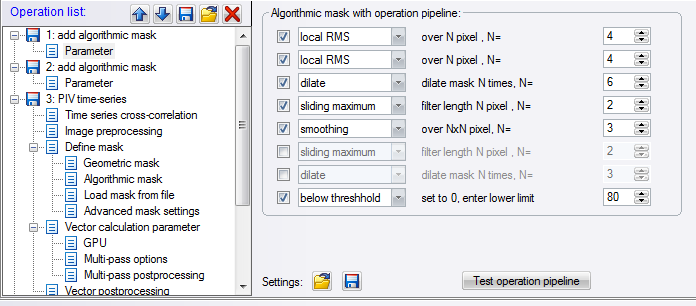
\includegraphics[width=\textwidth]{figures/Chapter_1/mask_1.PNG}
	\caption{Low intensity dynamic masking}
\end{figure}
\begin{figure}[H] %
	\centering%
  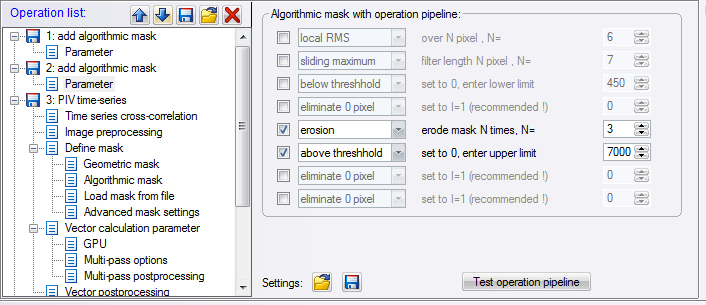
\includegraphics[width=\textwidth]{figures/Chapter_1/mask_2.PNG}
	\caption{High intensity dynamic masking}
\end{figure}
\begin{figure}[H] %
	\centering%
  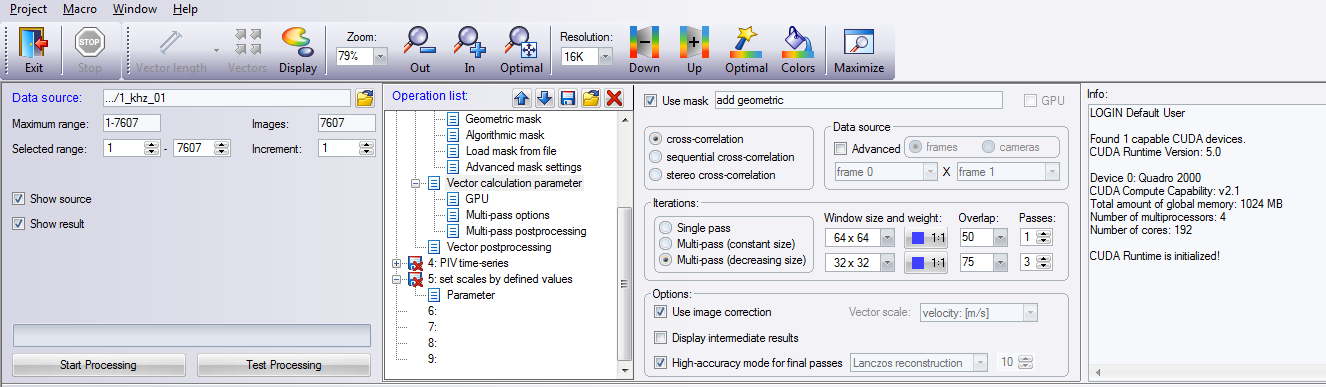
\includegraphics[width=\textwidth]{figures/Chapter_1/PIV-2.PNG}
	\caption{Cross-correlation settings}
\end{figure}